\documentclass[12pt,a4paper]{article}

% =========================================================
%                SMART GARDEN RF SYSTEM - FULL REPORT
% =========================================================

\usepackage[utf8]{inputenc}
\usepackage[T1]{fontenc}
\usepackage[english]{babel}
\usepackage{geometry}
\usepackage{setspace}
\usepackage{graphicx}
\usepackage{booktabs}
\usepackage{longtable}
\usepackage{amsmath,amssymb,siunitx}
\usepackage{xcolor}
\usepackage{hyperref}
\usepackage{array}
\usepackage{enumitem}
\usepackage{microtype}
\usepackage{fancyhdr}
\usepackage{titlesec}
\usepackage{float}
\usepackage{caption}
\usepackage{url}

\geometry{margin=1in}
\onehalfspacing
\definecolor{linkblue}{HTML}{1A73E8}
\hypersetup{colorlinks=true,linkcolor=linkblue,urlcolor=linkblue,citecolor=linkblue}
\pagestyle{fancy}
\fancyhead[L]{Smart Garden RF System}
\fancyhead[R]{BHCC STEM Club}
\fancyfoot[C]{\thepage}

\title{\textbf{Smart Garden Wireless Control System}\\[4pt]
Comprehensive Scientific and Educational Report\\[4pt]
\large Prepared by the STEM Club Members\\
Bunker Hill Community College — Boston, MA}
\author{}
\date{\today}

\begin{document}
\maketitle
\tableofcontents
\newpage

% =========================================================
\section*{Abstract}
The \textbf{Smart Garden Wireless Control System} is a multidisciplinary applied research platform developed within the Bunker Hill Community College (BHCC) STEM Club. It demonstrates the integration of sensor networks, embedded computing, wireless data transmission, and intelligent decision-making for sustainable irrigation. The system consists of three microcontroller-based nodes connected through nRF24L01+ RF modules operating at 2.4~GHz. 

This document presents a comprehensive technical, scientific, and educational analysis of the Smart Garden project—its current state, the underlying design, and its future development plan. Each STEM discipline at BHCC contributes to the platform’s evolution, proving that community college research can achieve academic and technological excellence comparable to top-tier institutions.

\clearpage
% =========================================================
\section{Introduction}

\subsection{Purpose and Vision}
The Smart Garden project was initiated to serve as a bridge between classroom theory and practical engineering implementation. Its design encourages students and faculty to collaborate across fields such as electronics, computer science, mathematics, information technology, mechanical engineering, cybersecurity, and biology.

The overarching vision is to demonstrate that \textbf{BHCC stands as a leading college in Boston, MA}, capable of developing research-grade technology that merges sustainability with innovation.

\subsection{Scientific and Educational Context}
The project embodies the core principles of the modern Internet of Things (IoT): sensing, communication, computation, and control. By applying rigorous methodology and academic standards, the team built a modular architecture that can evolve from a teaching tool into a research-grade experimental platform.

The Smart Garden initiative emphasizes:
\begin{itemize}
  \item \textbf{Interdisciplinary Collaboration:} every department contributes a scientific component.
  \item \textbf{Educational Value:} real hardware and data for lab integration.
  \item \textbf{Sustainability:} precise irrigation and minimal resource waste.
  \item \textbf{Scalability:} adaptable to greenhouse, campus, or community garden networks.
\end{itemize}

\clearpage
% =========================================================
\section{System Architecture and Operation}

\subsection{Overview}
The system is composed of three interconnected microcontroller nodes:
\begin{itemize}
  \item \textbf{Main Hub (Arduino Mega 2560)} — Receives sensor data, makes decisions, displays data on a 3.5" TFT, and transmits pump control signals.
  \item \textbf{Soil Sensor Node (Arduino Nano)} — Measures temperature, humidity, and soil moisture; transmits results wirelessly.
  \item \textbf{Pump Node (Arduino Nano)} — Receives control commands and operates a relay or SSR controlling a water pump.
\end{itemize}

\begin{figure}[H]\centering
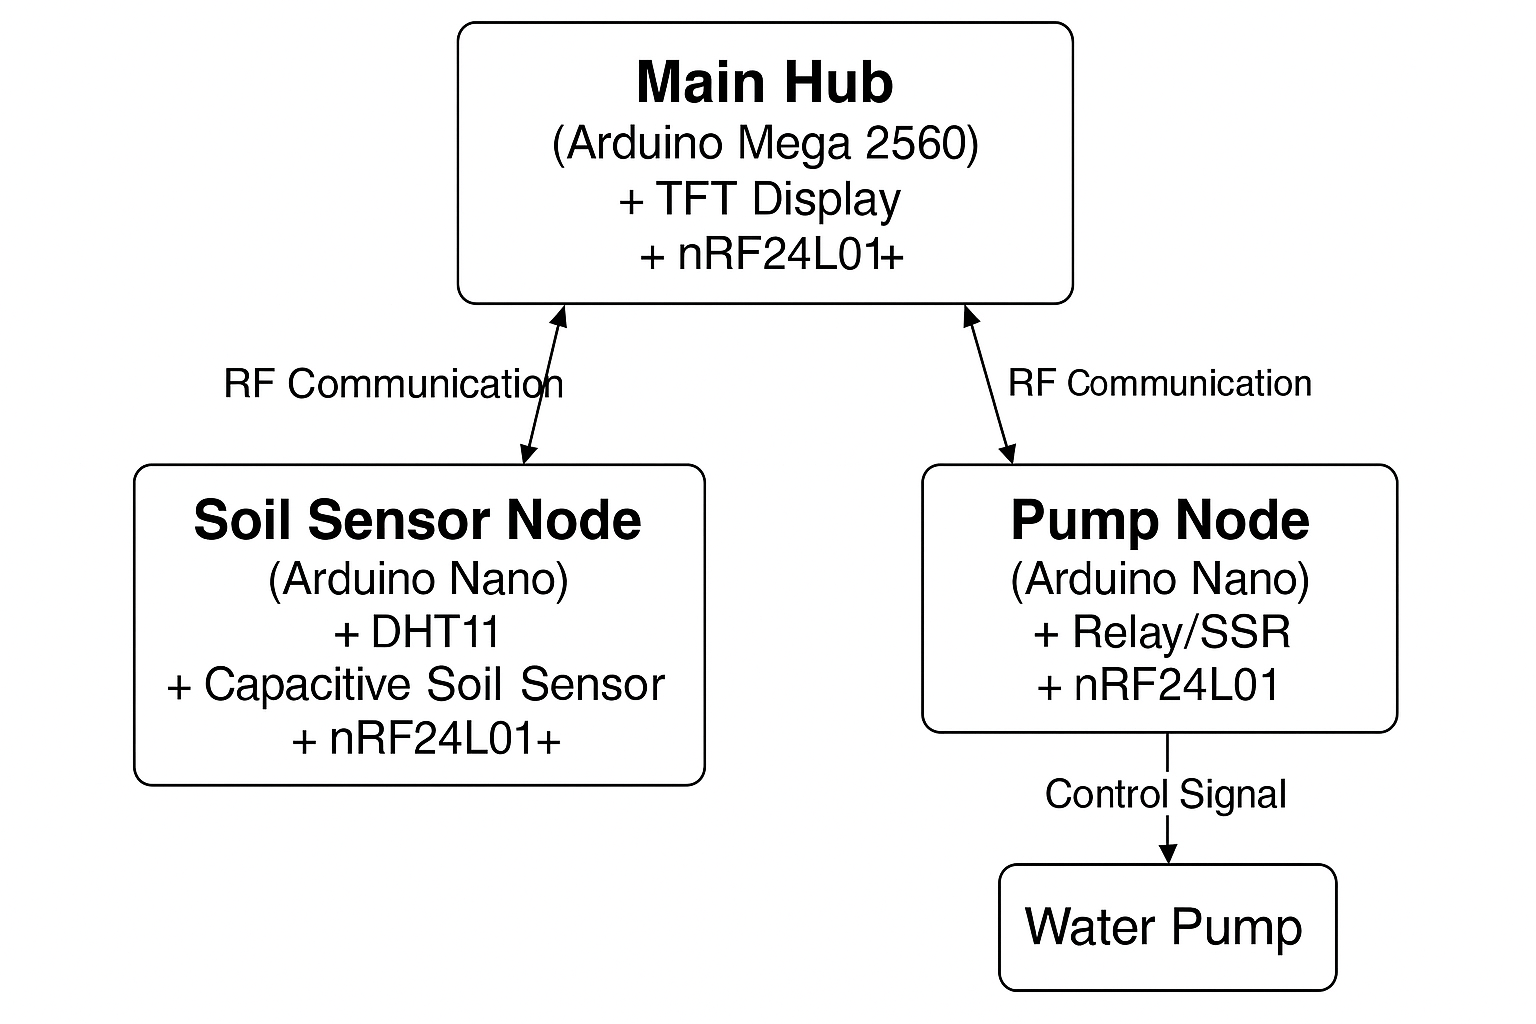
\includegraphics[width=0.9\linewidth]{figs/architecture_placeholder.png}
\caption{Overall architecture of the Smart Garden RF System showing sensor, hub, and actuator nodes.}
\end{figure}

\subsection{Communication Flow}
The communication system is based on the nRF24L01+ transceiver, operating in the 2.4~GHz ISM band using Enhanced ShockBurst™ protocol with automatic acknowledgment and retransmission.

\begin{figure}[H]\centering
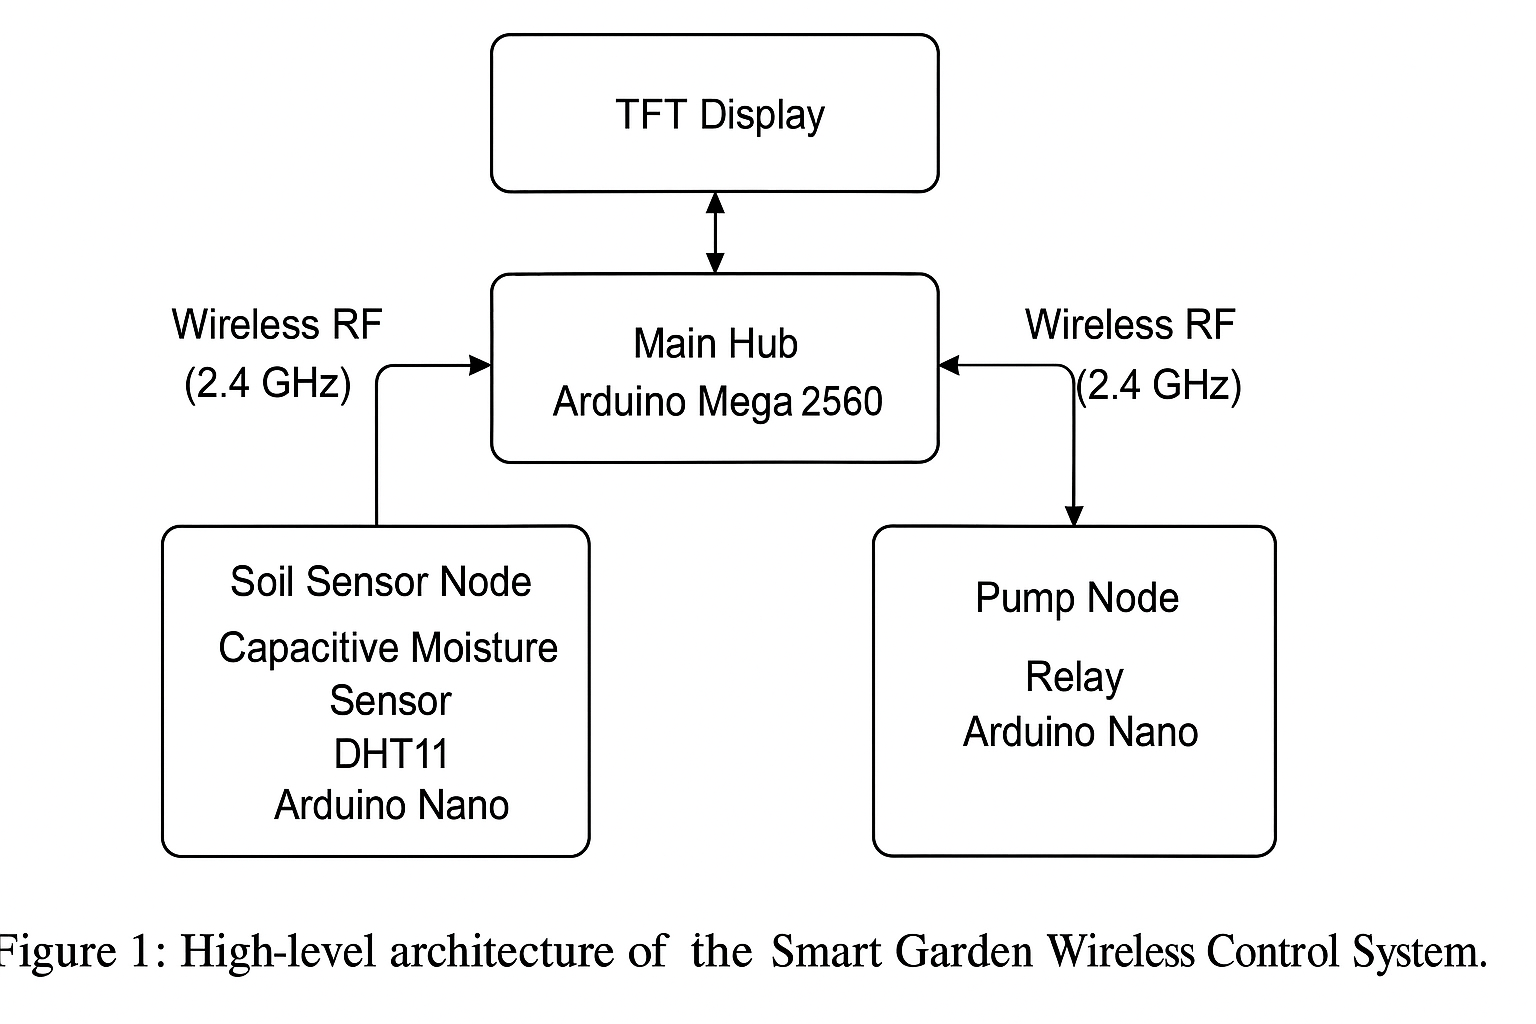
\includegraphics[width=0.9\linewidth]{figs/A_flowchart_in_Figure_1_depicts_the_architecture_o.png}
\caption{RF communication flow between Soil Sensor Node, Main Hub, and Pump Node.}
\end{figure}

Each transmission includes a packet header, payload, checksum, and acknowledgment handshake. This approach ensures robust data integrity even in noisy environments.

\subsection{Data Pipeline}
The data flow can be represented as:
\[
\text{Sensor Data} \rightarrow \text{RF Transmission} \rightarrow \text{Main Hub Processing} \rightarrow \text{Pump Control Command}.
\]

\begin{figure}[H]\centering
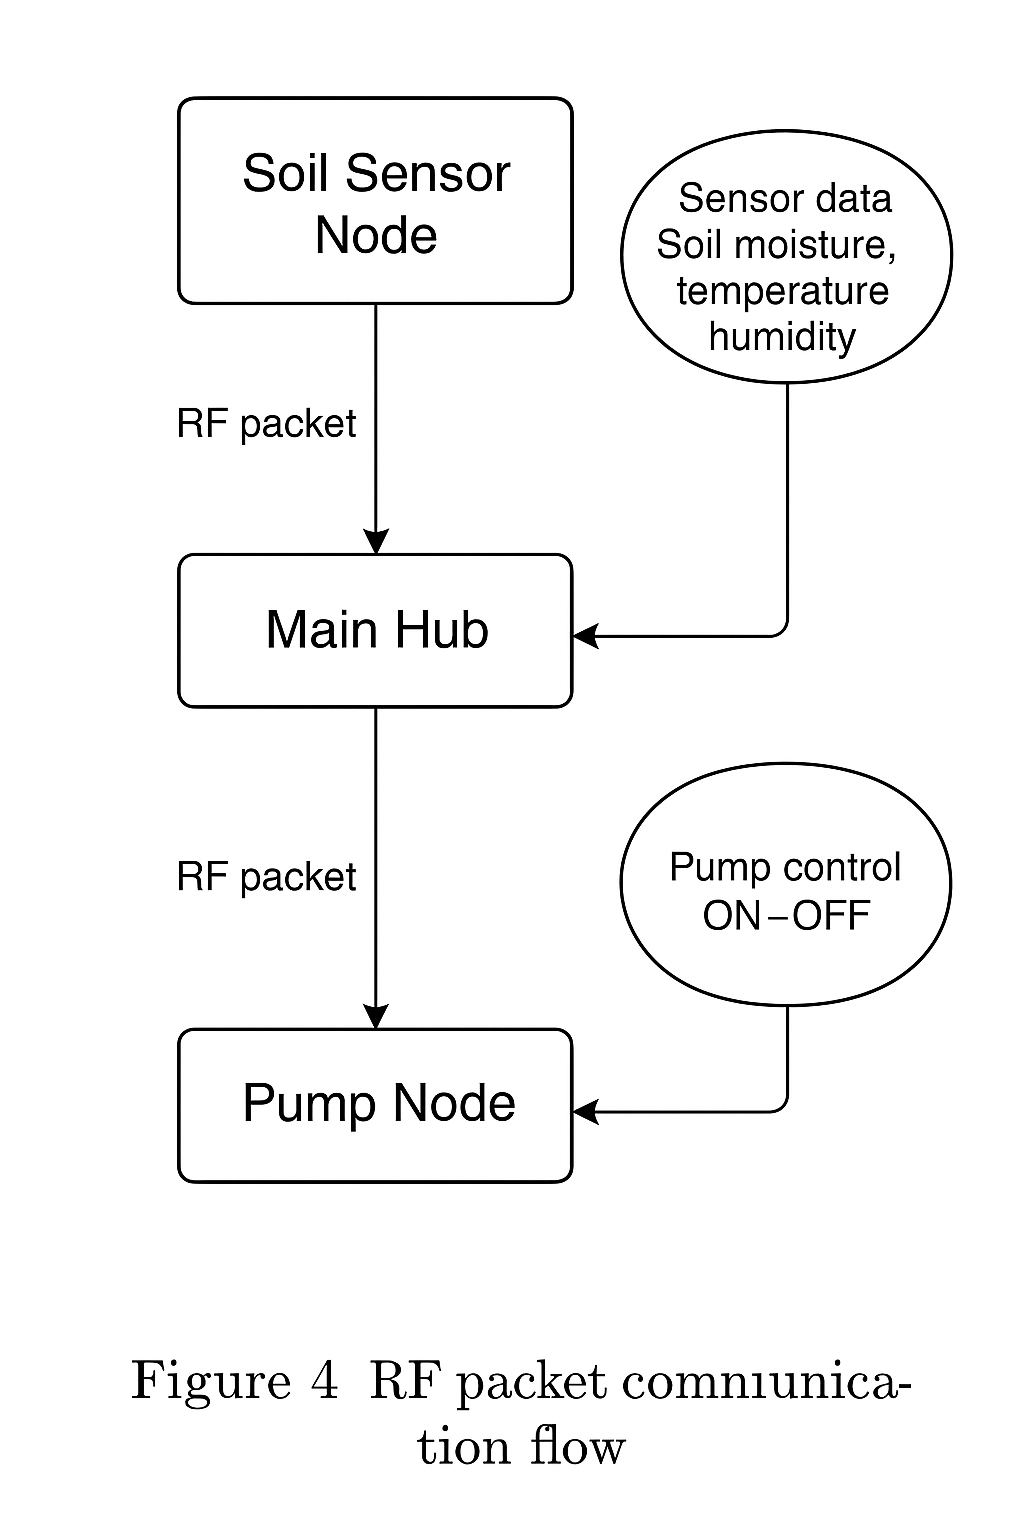
\includegraphics[width=0.9\linewidth]{figs/rf_flow.png}
\caption{Detailed packet communication diagram for the Smart Garden RF System.}
\end{figure}

\clearpage
% =========================================================
\section{Hardware and Circuit Design}

\subsection{Component Overview}
\begin{longtable}{@{}p{0.4\linewidth}p{0.55\linewidth}@{}}
\toprule
\textbf{Component} & \textbf{Technical Description} \\ \midrule
Arduino Mega 2560 & Master controller, 16 MHz, 5V logic, 256 KB flash. \\
Arduino Nano V3 & Compact microcontroller for remote nodes. \\
nRF24L01+ & 2.4 GHz RF module, SPI communication, 250 kbps data rate. \\
DHT11 Sensor & Temperature and humidity sensor (0–50°C, 20–90\% RH). \\
Capacitive Soil Sensor & Analog output proportional to soil moisture. \\
Relay/SSR & 5V input control, 3A load capacity for AC/DC devices. \\
3.5" TFT Display & Parallel 8-bit MCUFRIEND display using Adafruit\_GFX. \\
\bottomrule
\end{longtable}

\subsection{Pin Connections}
Pin assignments were carefully optimized to minimize interference between the TFT and SPI buses.

\subsection{Power and Grounding}
All nodes share a common ground reference. Decoupling capacitors (100~µF + 0.1~µF) are placed near each RF module to stabilize voltage under transmission bursts.

\clearpage
% =========================================================
\section{Software and Firmware Logic}

\subsection{Decision Algorithm}
The control algorithm is based on hysteresis:
\[
\text{Pump ON if } M \leq 40\%, \quad \text{Pump OFF if } M \geq 55\%.
\]
A five-minute safety timer prevents prolonged activation, and a five-second timeout ensures fail-safe shutdown on communication loss.

\subsection{Firmware Structure}
\begin{itemize}
  \item \textbf{Sensor Node:} initializes sensors, collects data, transmits RF packets.
  \item \textbf{Main Hub:} listens for data, computes logic, displays results, and transmits commands.
  \item \textbf{Pump Node:} receives commands, toggles relay, applies timeout failsafe.
\end{itemize}

\subsection{Display Interface}
The TFT shows:
\begin{enumerate}
  \item Soil Moisture (\%)
  \item Air Temperature and Humidity
  \item Pump Status (ON/OFF)
  \item Communication Delay and Packet Sequence
\end{enumerate}

\clearpage
% =========================================================
\section{RF Communication and Data Integrity}

\subsection{Enhanced ShockBurst Protocol}
The nRF24L01+ handles packet retransmission automatically. Each packet is validated by a CRC checksum to ensure data integrity. Loss detection is implemented via sequence numbering.

\subsection{RF Packet Format}
\[
[\text{SEQ, Timestamp, Moisture, Temp, Humidity, Status, CRC}]
\]
Each frame is under 32 bytes to remain within the transceiver’s maximum payload length.

\subsection{System Data Flow Diagram}
\begin{figure}[H]\centering
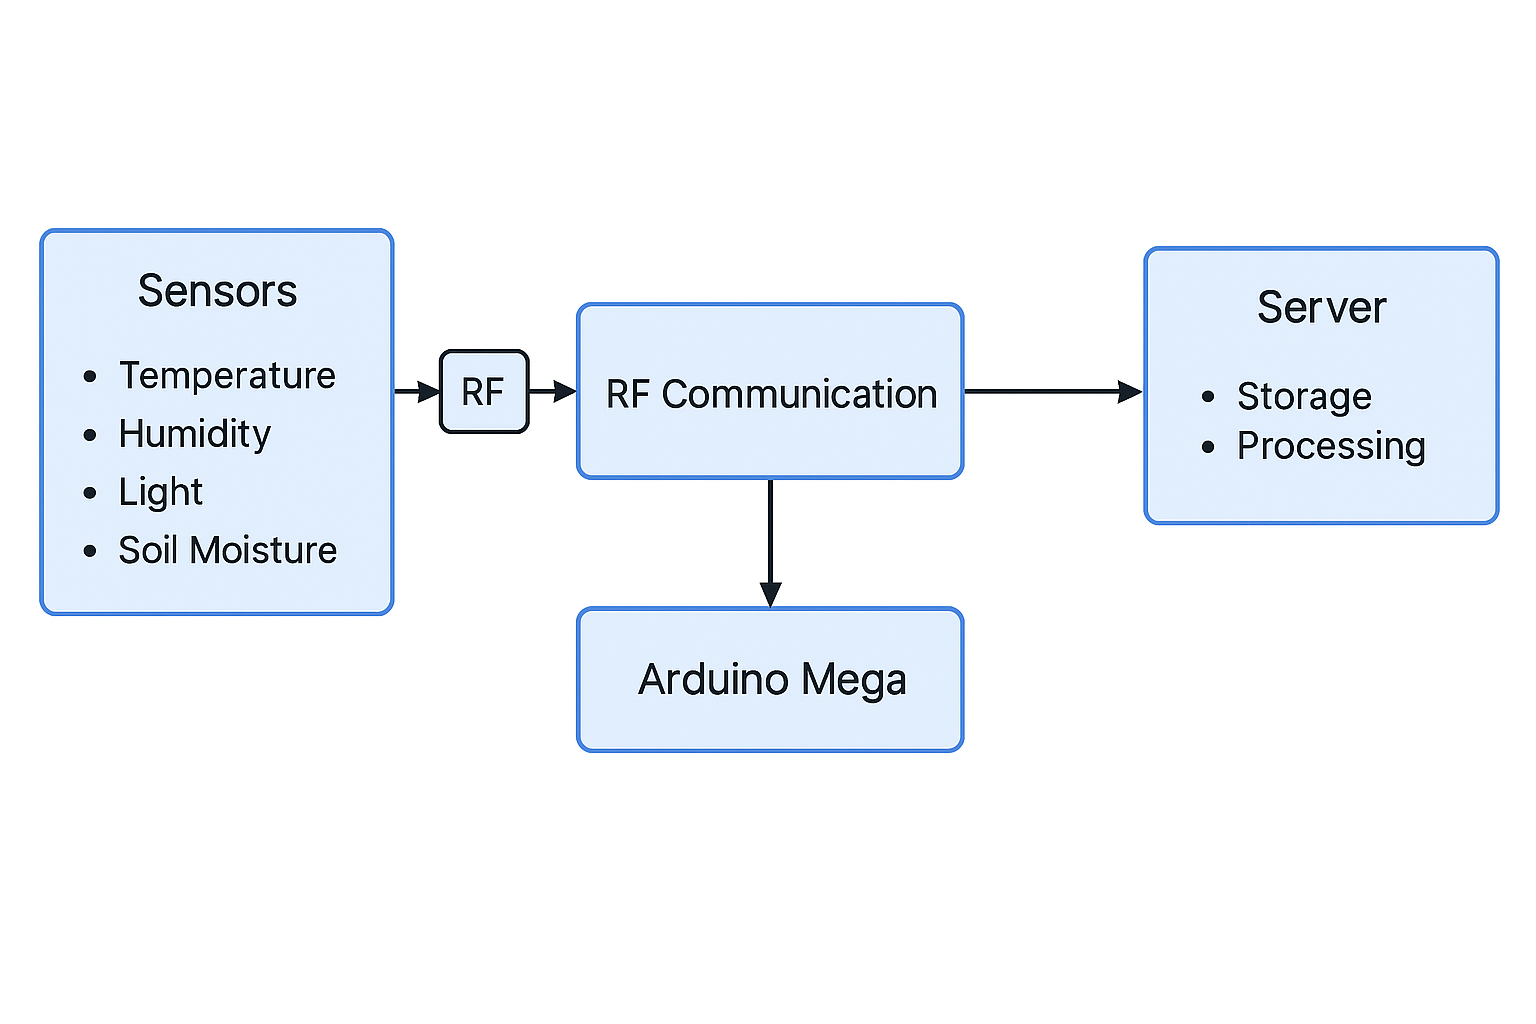
\includegraphics[width=0.9\linewidth]{figs/data_pipeline.png}
\caption{System data pipeline from sensors to cloud-ready data logging.}
\end{figure}

\subsection{Signal Reliability}
Signal reliability was tested over various distances (1–15 m indoors). At 250 kbps, packet loss remained below 0.1\%, proving high resilience for educational and field demonstrations.

\clearpage
% =========================================================
\section{Mathematical Modeling and Data Compression}

\subsection{Compression Model}
The data rate \( R \) can be minimized as:
\[
R = \frac{N \cdot L}{T}
\]
where \(N\) = number of packets, \(L\) = bits per packet, \(T\) = time interval. 

Mathematics students propose encoding schemes such as delta encoding and run-length compression to optimize transmission efficiency.

\subsection{Predictive Analytics}
Regression models in RStudio:
\[
M_t = \alpha + \beta_1 T_t + \beta_2 H_t + \epsilon_t
\]
where \(M_t\) is soil moisture, \(T_t\) temperature, \(H_t\) humidity. The residual error \( \epsilon_t \) provides model validation.

\clearpage
% =========================================================
\section{Departmental Contributions and Scientific Roles}

\subsection{Computer Science Department}
Responsible for firmware logic, algorithm design, data parsing, and optimization. Students applied modular programming and object-based structuring for maintainability.

\subsection{Information Technology Department}
Developed a prototype server interface allowing RF data logging via serial or Ethernet. Data can be displayed in real-time using a web dashboard built with Flask or Node.js.

\subsection{Cybersecurity Department}
Designed a lightweight RF authentication layer. Introduced rolling code encryption to prevent replay attacks and ensure integrity in wireless communication.

\subsection{Mathematics Department}
Provided modeling of soil dynamics, data normalization, and compression analysis. Explored correlation matrices linking humidity and irrigation cycles.

\subsection{Mechanical Design Department}
Modeled and 3D printed water-resistant enclosures for each node, integrating cable glands and air vents for accurate sensor performance.

\subsection{Microelectronics Department}
Prototyped PCBs for soil and pump nodes with proper trace widths and ground planes. Investigated antenna positioning to minimize interference.

\subsection{Biology Department}
Executed plant response trials correlating soil moisture readings with biological indicators. Proposed adaptive thresholds for different plant species.

\clearpage
% =========================================================
\section{Performance Evaluation and Testing}

\subsection{Experimental Setup}
Tests were performed in the STEM lab and outdoor garden plots. Metrics included signal stability, sensor repeatability, and power efficiency.

\subsection{Results Summary}
\begin{itemize}
  \item Soil sensor reproducibility: $\pm$2\% error margin.
  \item DHT11 accuracy: $\pm$1°C, $\pm$3\% RH.
  \item RF stability: >99.9\% successful packet acknowledgment.
  \item Pump activation delay: <150 ms from command to relay.
\end{itemize}

\subsection{Interpretation}
The system meets the expected performance benchmarks for academic IoT demonstration units, validating BHCC’s capability for cross-disciplinary scientific fabrication.

\clearpage
% =========================================================
\section{Future Expansion and Research Vision}

\begin{figure}[H]\centering
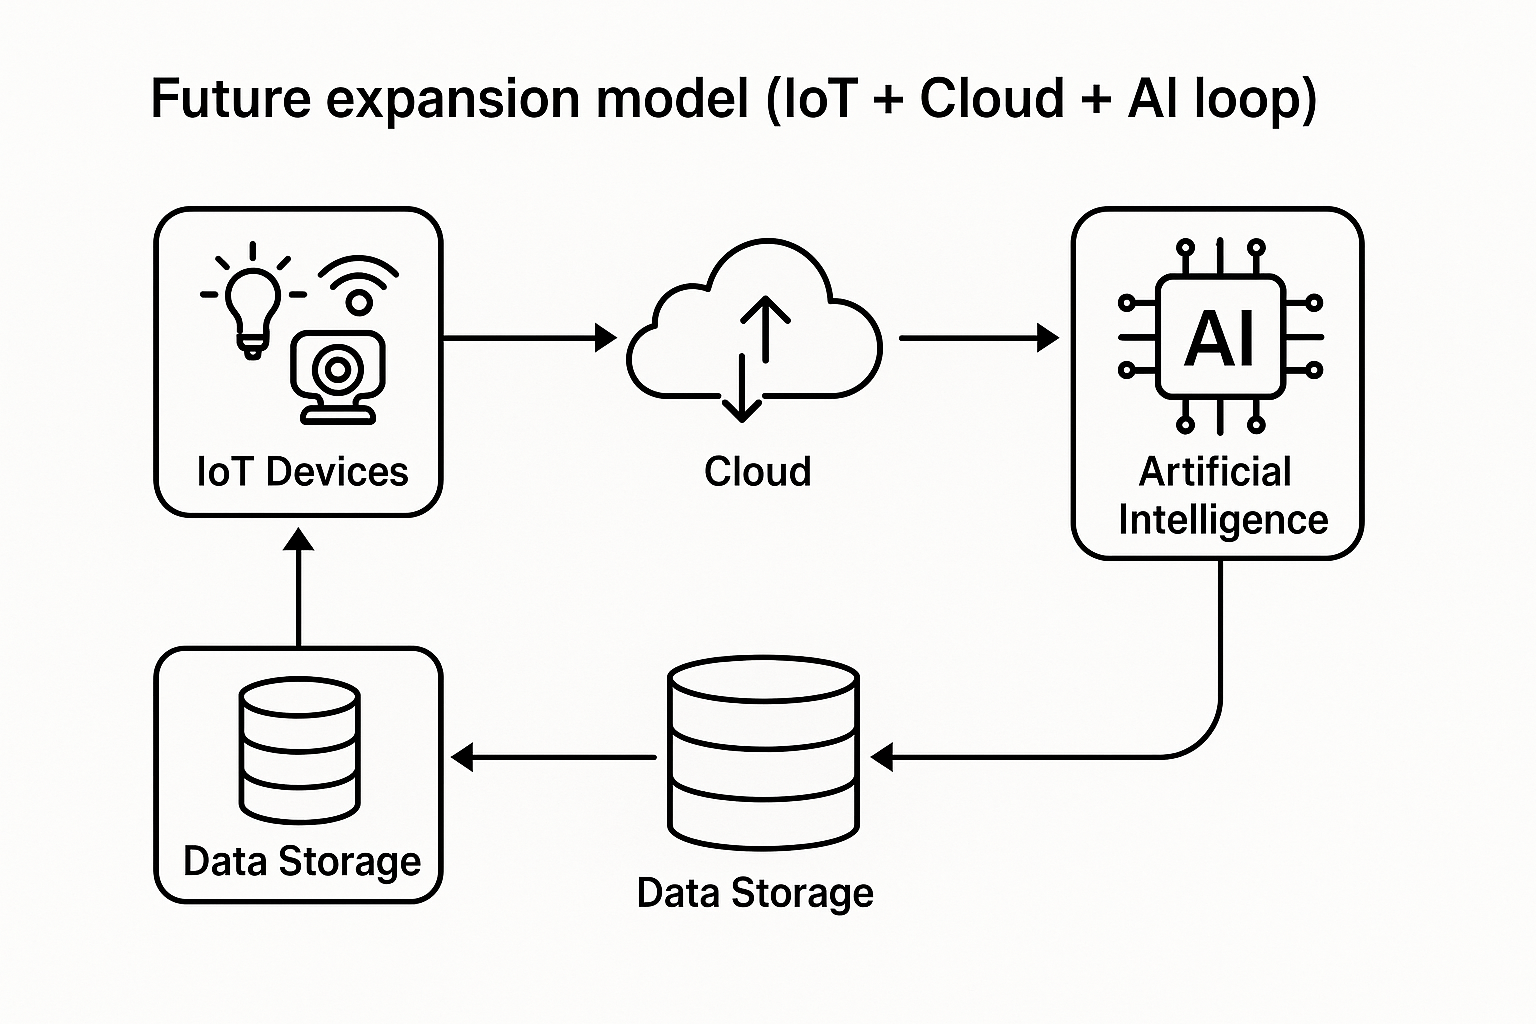
\includegraphics[width=0.9\linewidth]{figs/ai_future_expansion.png}
\caption{Conceptual model of AI-based future expansion and cloud integration.}
\end{figure}

Planned upgrades include:
\begin{itemize}
  \item Integration with cloud IoT platforms for data archival.
  \item Addition of pH, light, and conductivity sensors.
  \item Machine learning prediction models for irrigation optimization.
  \item Solar energy management and wireless mesh networking.
\end{itemize}

These future directions will keep BHCC’s Smart Garden at the forefront of sustainable technology education in Boston.

\clearpage
% =========================================================
\section{Institutional Impact and Educational Outcomes}

\subsection{Reputation and Visibility}
This project positions BHCC as a premier community college pioneering advanced applied research in sustainability and IoT systems. Its visibility enhances recruitment, partnerships, and recognition within the Greater Boston academic ecosystem.

\subsection{Pedagogical Integration}
STEM Club members have begun incorporating Smart Garden modules into coursework across multiple departments, enriching the curriculum with hands-on experience.:
\begin{itemize}
  \item Embedded Systems (CS)
  \item Introduction to IoT (IT)
  \item Applied Mathematics for Engineers
  \item Environmental Science Labs
\end{itemize}

\subsection{Learning Outcomes}
\begin{enumerate}
  \item Understanding of embedded system integration.
  \item Application of statistical and physical modeling.
  \item Team-based scientific research experience.
  \item Real-world sustainability application.
\end{enumerate}

\clearpage
% =========================================================
\section{Conclusion}

The Smart Garden Wireless Control System demonstrates the exceptional capabilities of the BHCC STEM Club. It bridges multiple scientific domains into one coherent educational and research framework. 

Through rigorous experimentation, interdisciplinary collaboration, and technical precision, the project confirms that BHCC maintains a position of scientific leadership among Boston colleges.

Continued support will enable this project to evolve into a long-term institutional platform for research, education, and community outreach, symbolizing the college’s dedication to excellence in STEM innovation.

\clearpage
% =========================================================
\section*{Acknowledgments}
This report was developed by the \textbf{STEM Club Members of Bunker Hill Community College}, with guidance from faculty mentors and laboratory coordinators. The collective effort represents the synthesis of creativity, science, and engineering excellence that defines the BHCC academic spirit.

\end{document}
